\chapter{Nuclear Astrophysics}
    \section{Solar Fusion Processes}
        \subsection{Overview}
            The proton-proton chain reaction is one of two known sets of nuclear fusions reactions in stars which convert hydrogen into helium. The PP Process dominates in stars with mass $<$ \(\textup{M}_\odot\). The CNO cycle dominates in stars with mass $>$ 1.3 \(\textup{M}_\odot\).
            
                 
                \begin{figure}[H]
                    \centering
                    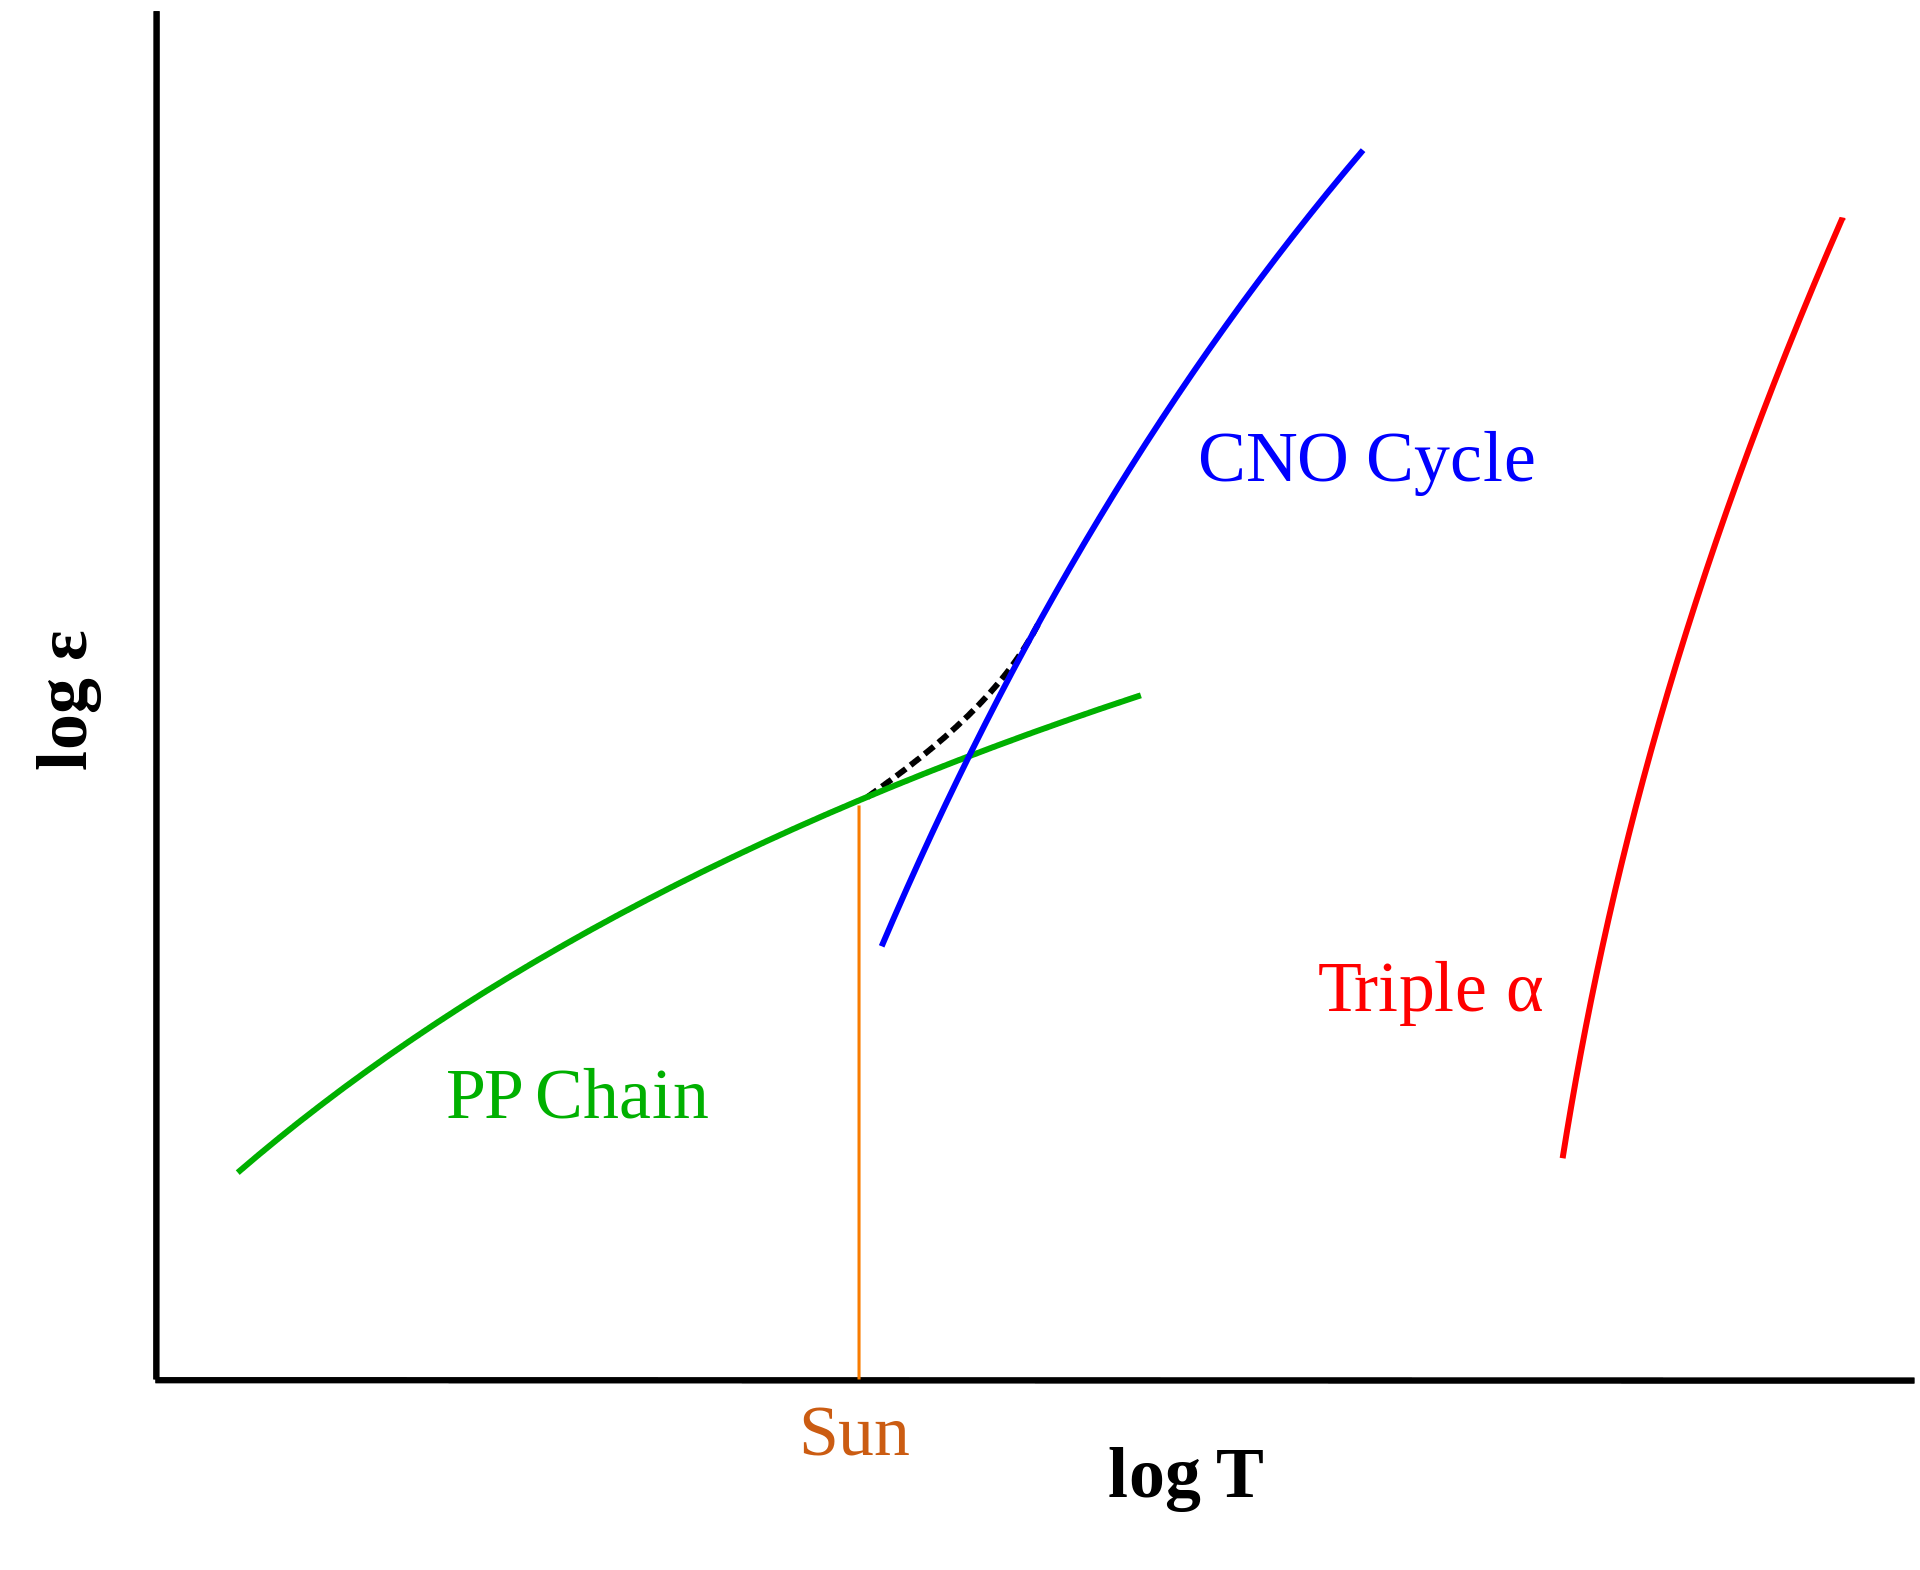
\includegraphics[width=8cm]{NuclearPhysics/modules/nuc-astro/pics/all-fusion-proc.png}
                \caption{Comparison of Fusion Processes in Stars vs. Temp}
                \end{figure}       


            \begin{figure}[H]
                \centering
                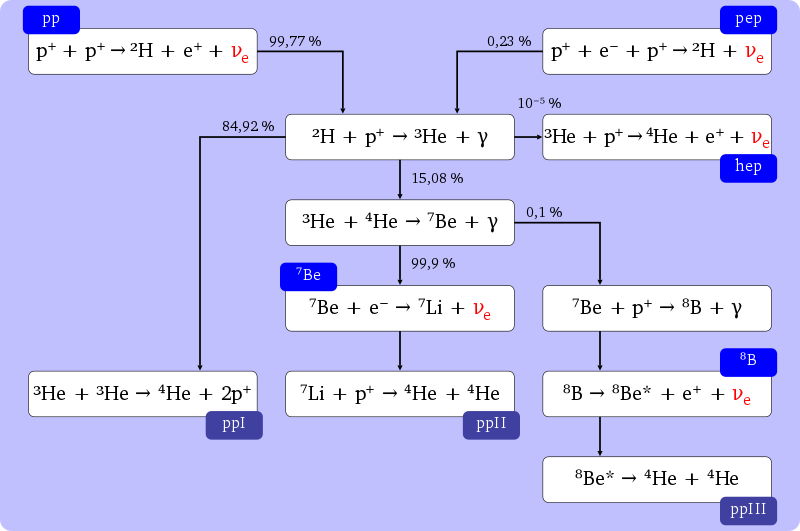
\includegraphics[width=10cm]{NuclearPhysics/modules/nuc-astro/pics/overview-solar-fusion-change.png}
            \caption{Summary of Fusion Processes}
            \end{figure}

           
    
        \subsection{PP Process}
                \subsubsection{Overview}
                    \indent  Proton-proton fusion can occur only if the temperature is high enough for protons to overcome the Coulomb barrier to get close enough. Di protons are the much more common result of proton-proton reactions within the star, which almost immediately decay back into protons. Based off of these reaction rates, the sun lifetime should be $sim$ 10 billion years. Due to quantum mechanical tunneling, protons can fuse at a lower temperature than classically predicted. In 1939 Hans Bethe proposed positron emission converting a proton into a neutron briefly to form deuterium. Bethe later won the Nobel prize in 1967 for general work in stellar nucleosynthesis.
               
                
                            

            \begin{figure}[H]
                \centering
                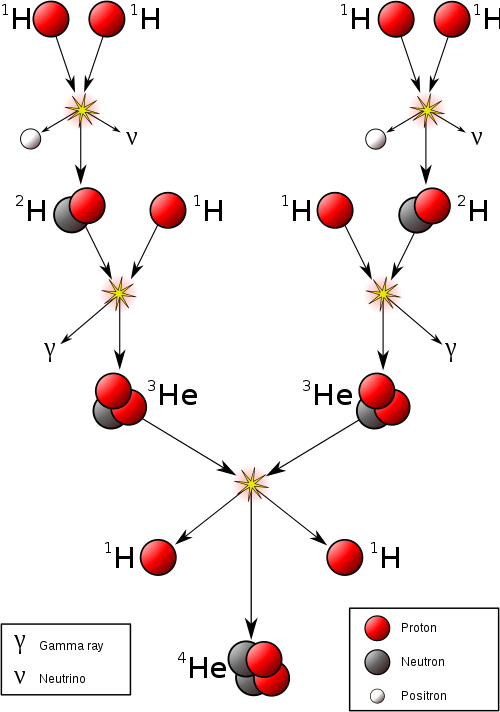
\includegraphics[width=5cm]{NuclearPhysics/modules/nuc-astro/pics/pp-branch1-rxn.png}
            \caption{PP-1 Chain Diagram}
            \end{figure}
                
                \subsubsection{The PP Chain}
                    \indent In words, the pp chain is:\\
                    \newline
                    Fuse two protons into deuterium. One proton undergoes beta plus decay, converting into the needed neutron and emitting a positron and electron neutrino.The emitted positron will annihilate with an electron to produce two gamma rays, giving a total Q value of 1.442 MeV. This step is rate limiting as it is mediated by the weak force. The average proton waits 9 billion years before it fuses with another proton. This cross section cannot be measured experimentally due to these long time scales.\\
                    \newline
                    Fuse the deuterium with a proton to make helium 3, and emit a gamma. This is a strong process, so is extremely fast. A deuterium nucleus exists for only 4 seconds before conversion to He3.\\
                    \newline
                    Once Helium-3 is made, there are four paths to generate Helium-4:\\
                    \newline
                    \indent p-p I \indent - \indent Fuse 2 helium-3 together to make Helium-4 and 2 protons \indent 83.3\% BR\\ Q value of last step 12.86 MeV. Overall ppI chain releases 27 MeV, 2 percent is lost to neutrinos. Dominant at temps of 10 to 14 Mega Kelvin.\\
                    \newline
                    \indent p-p II \indent - \indent Fuse 2 helium-3 together to make Helium-4 and 2 protons \indent 16.68\% BR\\ Also called lithium burning. He-3+He4 to Berylium7 plus gamma, Berylium7 + e- to Lithum 7 + electron neutrino and 0.9 MeV 80\% of the time, 0.4 MeV 20\% of the time, Lithum 7 plus proton to two He-4. Dominates between 14 to 23 MegaKelvin. \\
                    \newline
                    \indent p-p III \indent - \indent Fuse 2 helium-3 together to make Helium-4 and 2 protons \indent 0.02\% BR\\ He3 + He4 to Be7 and gamma, Be7+proton to B8 and gamma, B8 to Be8 and positron and electron neutrino, Be8 to 2 heliums. Dominate process if temperature over 23 Megakelvin. Very important process for resolving the solar neutrino problem as it generates neutrinos up to 14 MeV in energy. \\
                    \newline
                    \indent p-p IV \indent - \indent Fuse 2 helium-3 together to make Helium-4 and 2 protons \indent extremely rare - 0.3 ppm predicted\\ Direct capture of a proton by helium 3 to yield helium 4, would release neutrino up to 19 MeV in energy.
                
                \subsubsection{PEP reaction}
                    \indent The Proton-Electron-Proton is a reaction for production of deuterium via electron capture:\\
                    \newline
                    $^1H + e^- + ^1H \longrightarrow ^2D^+ + \nu_e$\\
                    \newline
                    \indent The frequency of PEP vs pp reaction is about 1 to 400, but the electron neutrino from this reaction is far more energetic at about 1.44 MeV compare to 0.42 MeV pp reaction neutrinos. Borexino detected this line of 1.44 MeV neutrinos in 2012. 
                    
        \subsection{CNO Cycle}
            \indent Reaction converting hydrogen to helium, using CNO as catalysts. Dominant for starts 1.3 times the mass of the sun. Dominant mode of main-sequence energy generation in stars larger than the Sun. The net reaction still fuses 4p →alpha, but requires carbon nuclei as a catalyst (so it can only happen after the first generation of stars died and expelled the carbon they produced). 
            
            Sun temperature is about 15 million K, only 2 \% of the He4 in the sun is produced from the CNO cycle. 
            
            The cycle goes:\\
            \newline
            C-13, + p = N-14, + p = O-15 - $e^+ \nu_e$ = N-15, + p =  He4 \& C-12, + p = N-13, -  $e^+ \nu_e$ = C-13\\
            \newline
            In words, we start with C-13, capture 2 protons, beta+ decay, add 2 protons, beta+ decay, etc. Overall we capture 4 protons and beta+ decay twice. The He-4 is emitted on adding a proton to N-15. Each reaction relases between 2 and 8 MeV of energy as gamma rays. Emitted neutrinos have energy ranges varying up to a couple MeV. Rate limiting steps is proton capture events. \\
            There are other branches for CNO (CNO-II, III, and IV) as well as Hot CNO cycles (where proton capture is no longer rate limiting) but not discussed here, see \href{https://en.wikipedia.org/wiki/CNO_cycle}{here} for more. As a last note, CNO is important as it predicts proportions of elements to be found in stars, which can then be measured. 
            
                        
            \begin{figure}[H]
                \centering
                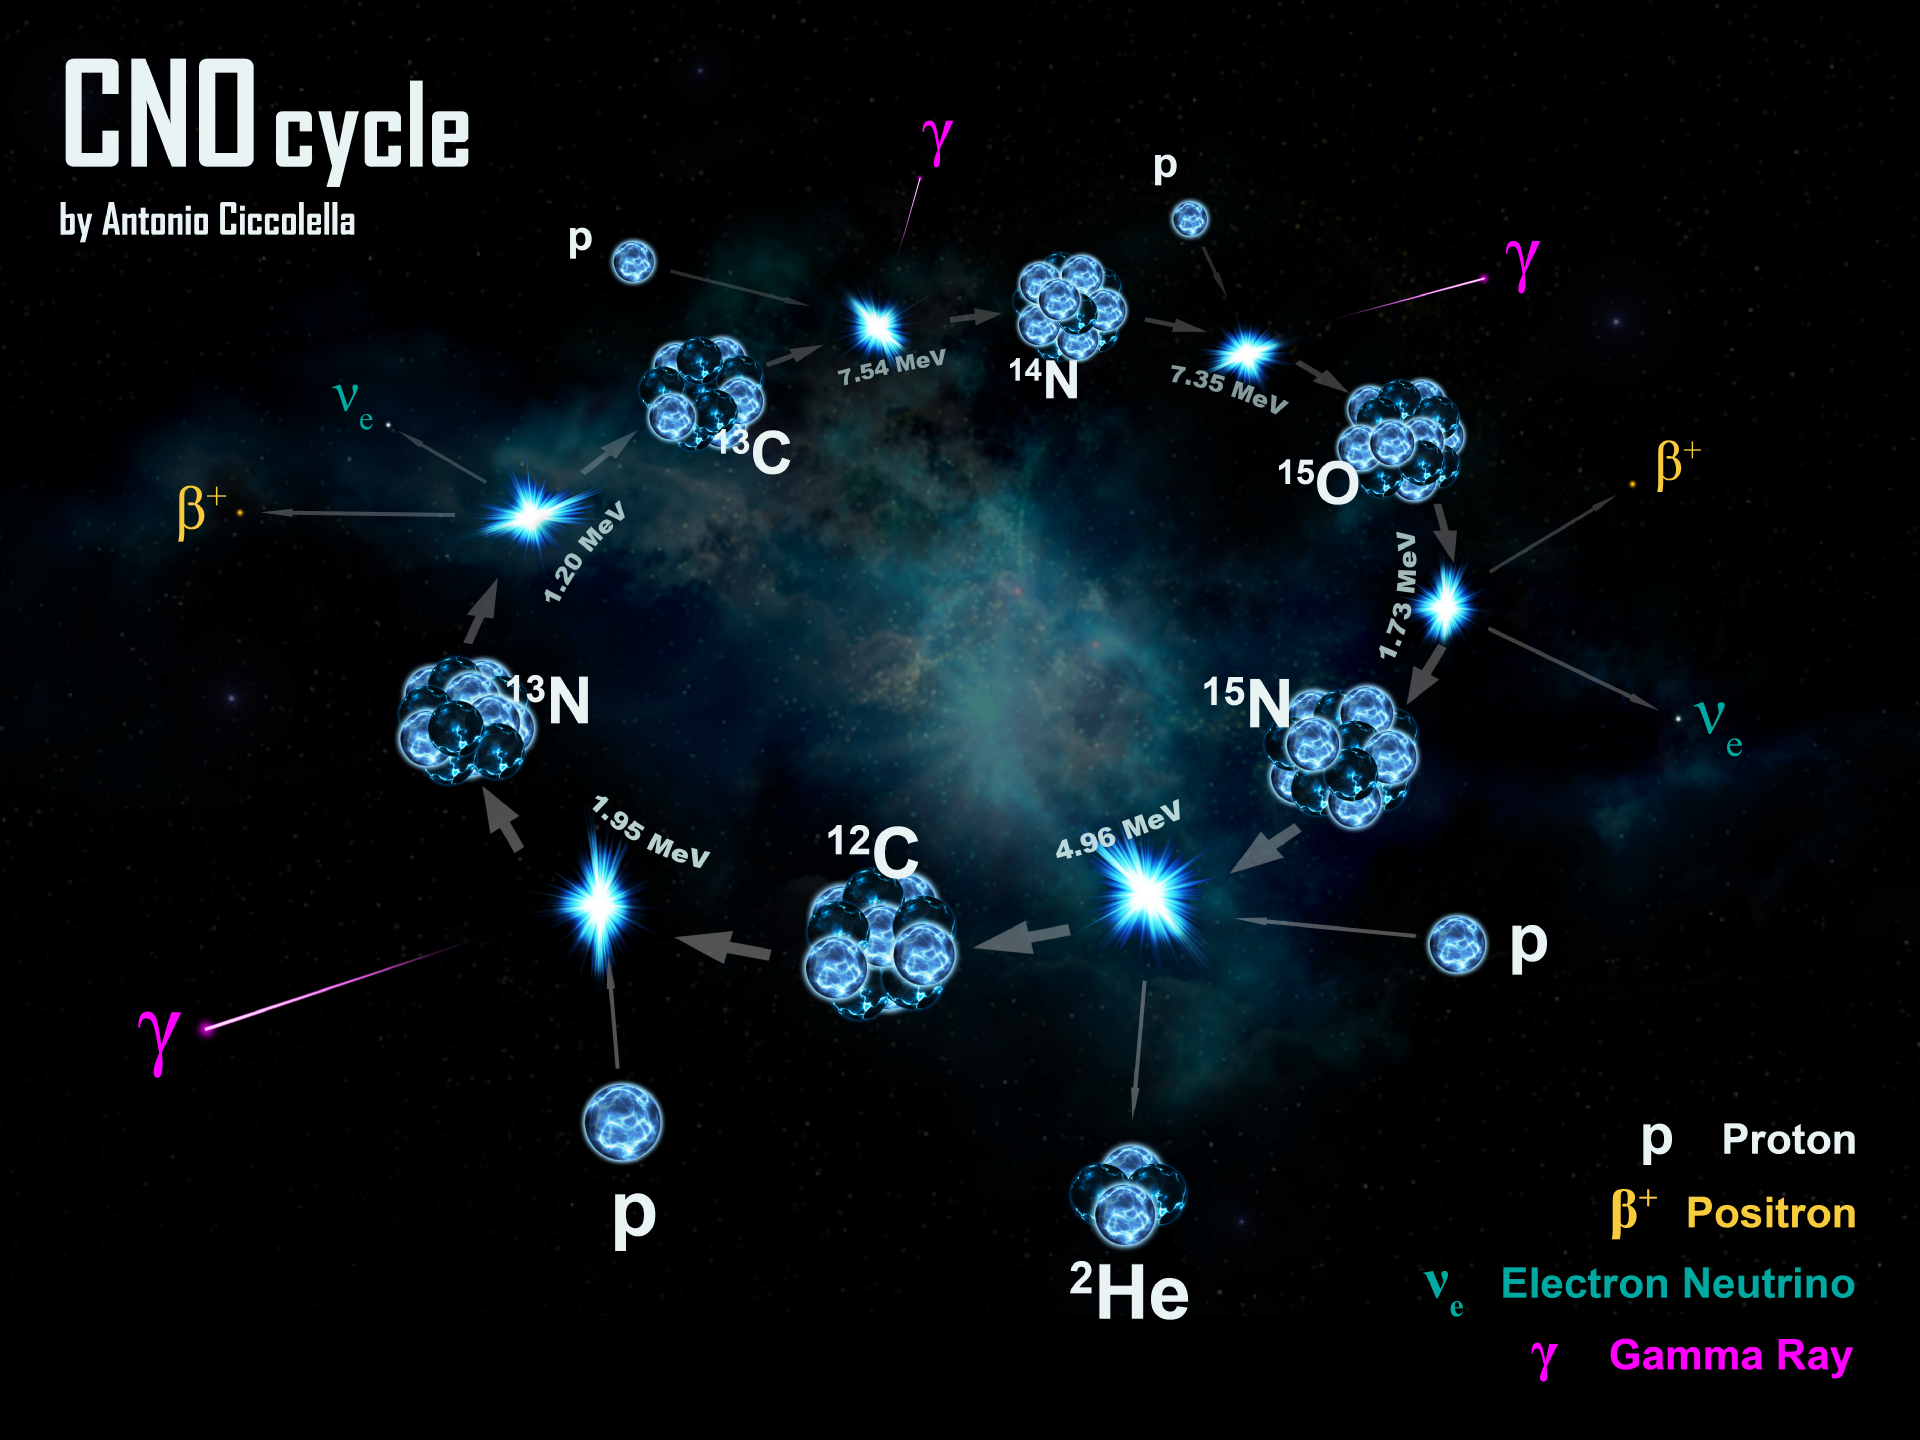
\includegraphics[width=8cm]{NuclearPhysics/modules/nuc-astro/pics/CNO-best.png}
            \caption{CNO Cycle Diagram}
            \end{figure}
            
        \subsection{Triple Alpha Process}
            The triple alpha process fuses three He4 atoms into carbon. The reaction is:\\
            \newline
            He4 + He4 = Be8, + He4 = C12.\\
            \newline
            The half life of Be8 is only $1x10^-16$ s, so this is the rate limiting step. Triple alpha only starts becoming appreciable at temperatures of 100 million K. Importantly, the step combining Be8 and He4 to C12 goes to an excited state of carbon-12, a resonance known as the Hoyle state - a 7.66 MeV $0^+$ resonance, which greatly increases the probability that an incoming alpha particle will combine with Be-8 to form carbon. \\
            As a side note, the power released by the triple alpha process is proportional to temperature to the 40th power, and density squared, while pp-chain is proportional to temp to the fourth, and CNO at temp to the 17th, while both are linearly proportional to the density. 
             

            \begin{figure}[H]
                \centering
                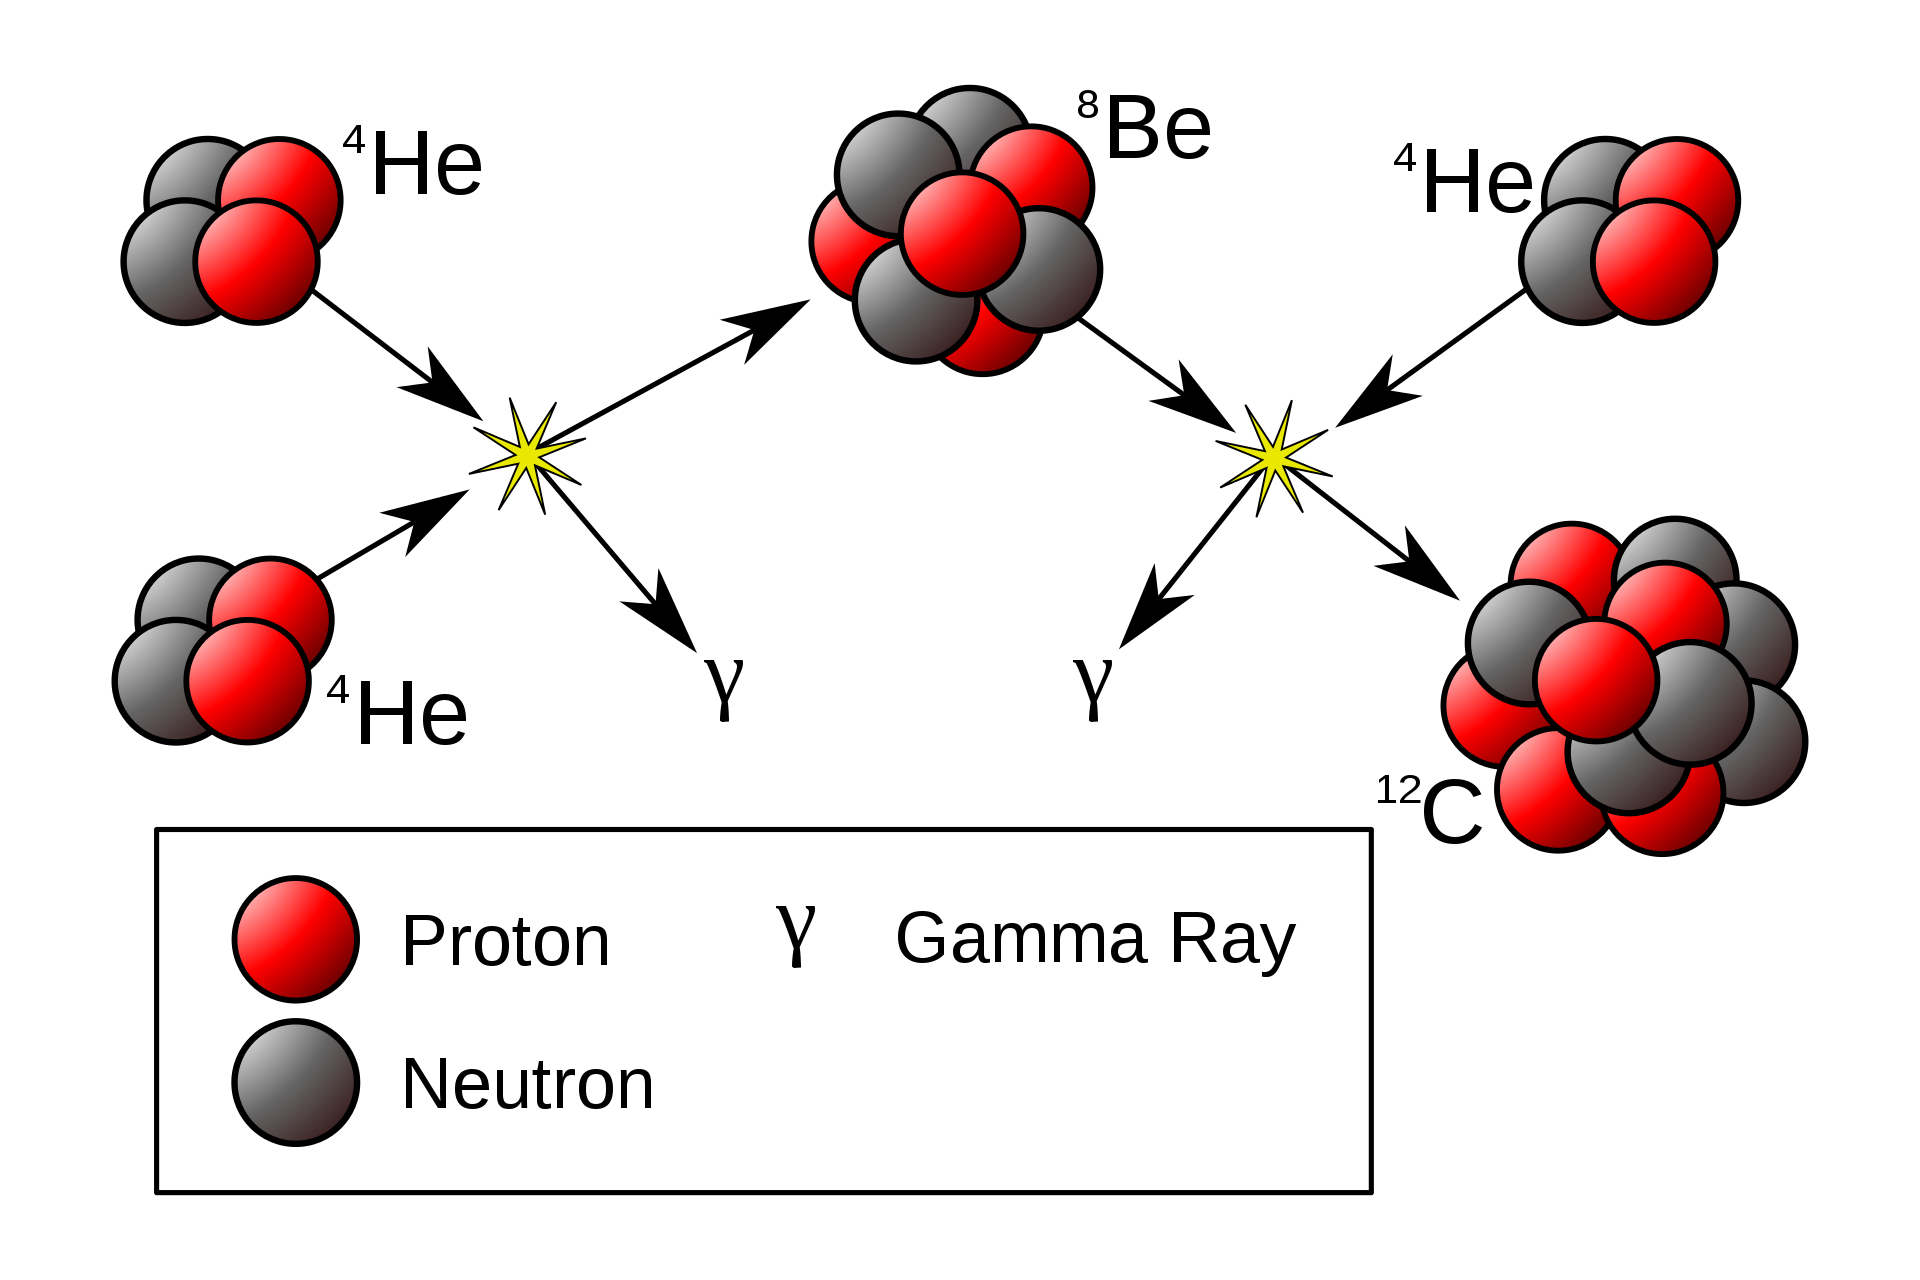
\includegraphics[width=9cm]{NuclearPhysics/modules/nuc-astro/pics/triple-alpha.png}
            \caption{Triple Alpha Process Diagram}
            \end{figure}
            
            
            
            Heavier elements up to iron 56 are made in the alpha (ladder) process, where He4 combines with elements and releases a $\sim$ 5 MeV gamma. Note that this alpha process makes almost all the even elements. 
           
            \begin{figure}[H]
                \centering
                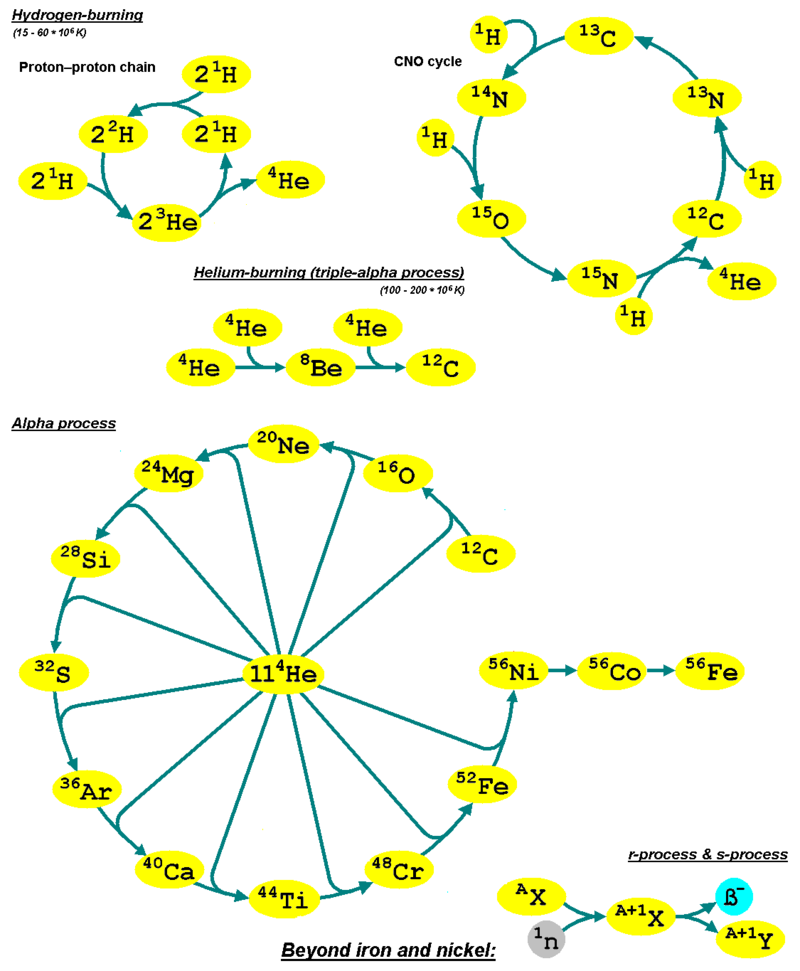
\includegraphics[width=8cm]{NuclearPhysics/modules/nuc-astro/pics/alpha-ladder-process.png}
            \caption{Alpha Ladder}
            \end{figure}
    \section{Elements Heavier than Iron}
        
            \begin{figure}[H]
                \centering
                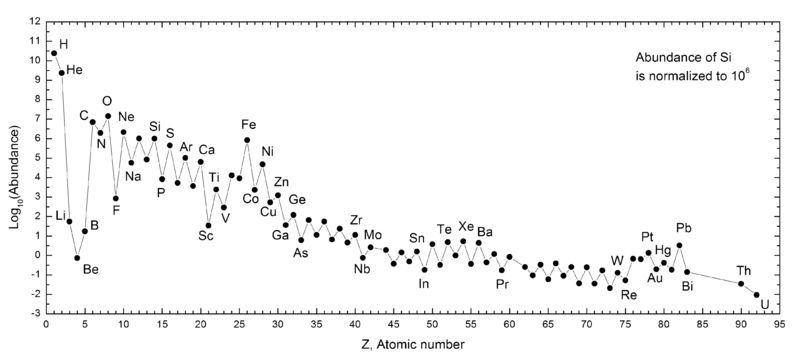
\includegraphics[width=11cm]{NuclearPhysics/modules/nuc-astro/pics/elemental-abundances-in-universe.png}
            \caption{Abundance of Elements in the Universe. Notice even-odd substructure.}
            \end{figure}
            
            Elements heavier than Iron are made predominantly by two processes - R process and S process. There is also the P- process.
    
        \subsection{R Process}
            r-process: neutron capture rate is rapid compared to beta-decay rate, so nuclei move far from stability toward the neutron drip line, eventually beta-decaying back to stability. Probably occurs predominantly in binary neutron-star mergers, i.e. kilonovae. Likely produces most of the elements near the neutron-rich side of the valley of stability. Microsecond timescales.
        \subsection{S Process}    
            s-process: neutron capture rate is slow compared to beta-decay rate, so nuclei move upward in mass, along the valley of stability. Probably occurs in large stars near the ends of their lives. Likely produces most of the elements near the center of the valley of stability above iron. Kilo-year timescales = $10^{11}$ seconds = $10^{17}$ microseconds.
        \subsection{P Process}
            p-process: invoked to produce certain neutron-deficient (proton rich) stable isotopes. Likely the result of (gamma, n) and (p, alpha) reactions in supernova shocks.)
    \section{Timeline of Universe}
        \subsection{Timeline Overview}
            \begin{table}[H]
                \centering
                    \begin{tabular}{llll}
                        \textbf{Epoch}       &       \textbf{Time}        &       \textbf{Temp}        &       \textbf{Description}\\
                        Plank       &       -43 s       &       19 GeV      &       quantum gravity\\
                        Grand Unification & -36 s       &       16 GeV      &       Three forces unified\\
                        Inflation       &   -32 s       &       9 GeV (22 K)      & Inflation, strong force decouples\\
                        Quark       &       -6 s        &       200 MeV     &       QGP \\
                        Hadron      &       1 s         &       1 MeV       &       Hadrons form\\
                        Neutrino Decoup.    & 1 s       &       1 MeV       &       Neutrinos decouple\\
                        Lepton      &       10 s        &       100 keV     &       Leptons and anti-lept in equil.\\
                        BBN         &       100 s       &       1 keV       &       He4, He3, Li7, D, form\\
                        Photon      &       370 kY      &       keV to 0.4 eV      &       plasma, no atoms\\
                        Recombination &     370 kY      &       0.4 eV      &       Atoms form, CMB set\\
                        Dark Ages   &       150 MY      &       60 K        &       No stars, no visible light\\
                        Stars       &       400 MY      &       60 K        &       Stars formed\\
                        Reionization &       1 GY        &       20 K        &       Hydrogen reionized        \\
                        Present     &       14 GY       &       2.7 K       &       Universe 46 GLY radius\\
                    \end{tabular}
            \end{table}
            
            
                  
            \begin{figure}[H]
                \centering
                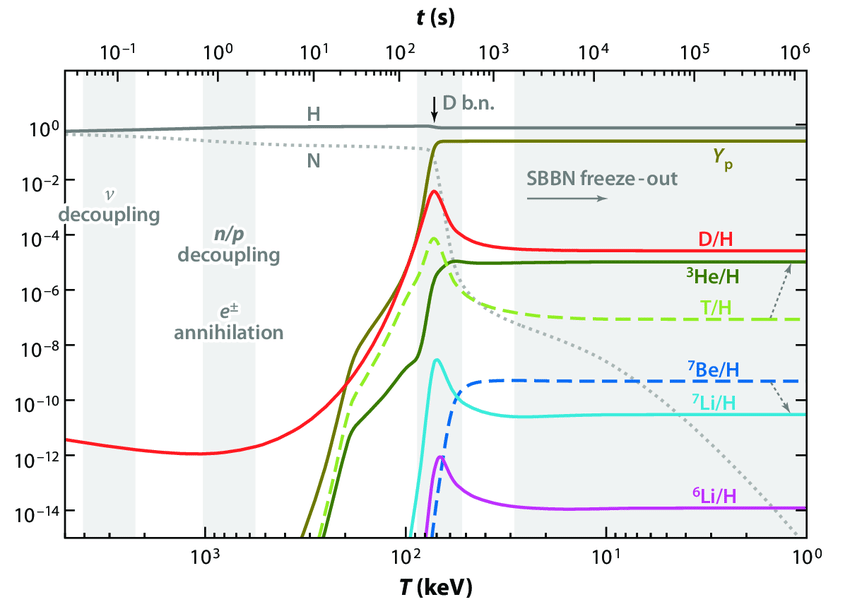
\includegraphics[width=11cm]{NuclearPhysics/modules/nuc-astro/pics/element-abundances-vs-temp.png}
            \caption{Abundance of Elements vs. Universe Time}
            \end{figure}
            
            Notes: Big Bang nucleosynthesis yields over time. Proton/neutron abundances were almost identical until the temperature fell below 1 MeV (corresponding to the Q-value for neutron decay, or the energy of the electron required to convert a proton into a neutron). Deuterium could only start to form when the temperature fell below ~2 MeV (binding energy of deuteron). Reaction rates quickly dropped as the temperature fell below ~100 keV (i.e., the reaction thresholds).
            
        \subsection{Big Bang Nucleosynthesis}
            Happened about 3 minutes after Big Bang, was when neutron and proton fused to make deuteiurm, He4 - 75\% Hydrogen, 25\% Helium, number of gluons to number of bayrons is 2*10$^9$. The Sakharov conditions describe necessary requirements to make the baryon - anti-baryon assymmetry, which are:\\
            1 - Baryon number violation\\
            2 - C and CP violation \\
            3 - Interactions outside of thermal equilibrium\\
            \\
            The proton to neutron ratio was about 7 when nucleosynthesis began. Also made some Li7. BBN - based on temperature and thermodynamics, there were 7 protons for every neutron. at the start of nucleogenesis. Helium 4 couldn't form readily because it needs deuterium as an intermediate, but temperature was above deuterium binding energy, this is called the deuterium bottleneck. Once temperature dropped low enough, a burst of element formation occurred. By 20 minutes after the big bang, universe was too cool for fusion, and nearly fixed abundances of elements. There are no stable nuclei with mass numbers five or eight. 
        
        
            The dynamics of what happened between 100M year and now is very sensitive to nuclear properties, specifically very neutron rich nuclei.
    
        \subsection{Measuring the Age of the Universe}
        Age of universe is calculated by measuring the Hubble Constant, which describes the expansion rate of the universe. Propagate it back to 0 size, and you get the life time. 
            
            \href{https://www.youtube.com/watch?v=TtIeozyQ3Is}{Nuclear Fusion in Stars Video That I Haven't Had Time to Watch}
            

    \section{Studying Nuclei Far From Stability}
        Why study this? As we get close to neutron drip line, binding energies are only on order of 100s of keV, instead of the usual several MeV per nucleon. Thus we can study pairing interactions in weakly bound systems. Also get exotic systems such as Li-11. 
             
            \begin{figure}[H]
                \centering
                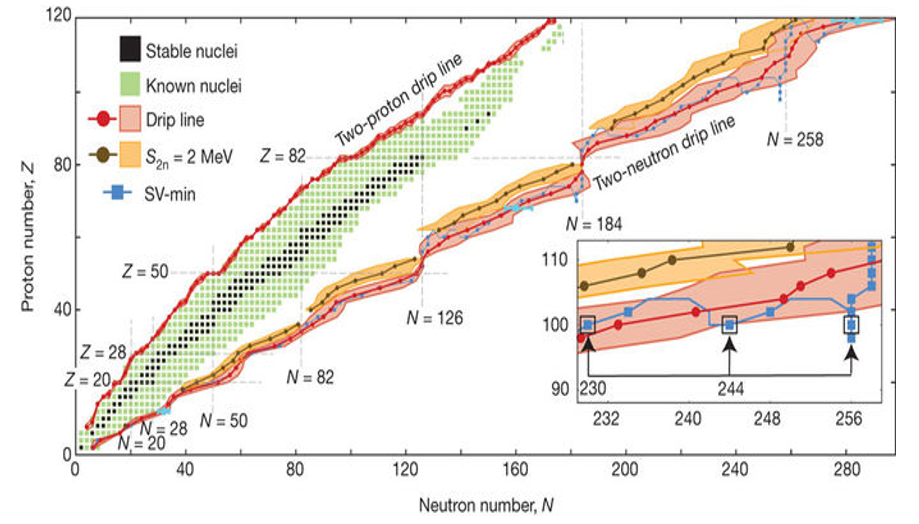
\includegraphics[width=11cm]{NuclearPhysics/modules/nuc-astro/pics/isotope_table.PNG}
            \caption{Table of Nuclides}
            \end{figure}
            
            Notes: no stable nuclei with masses 5 or 8, so lithium/beryllium abundance is low. Note the peaks near Z = 8, 26, 82 due to magic numbers/shell closures.
   
        Note: Where does FAIR fit into this? and the other Michigan accelerator?
        FRIB ISOLIDE
        \subsection{Projectile Fragmentation}
            Shoot a high energy (50-500 MeV/A) heavy ion beam on a thin target\\
            Various fragements with high velocity are produced\\
            Separate out fragemnts and made a radioactive beam\\
            
            
            \begin{figure}[H]
                \centering
                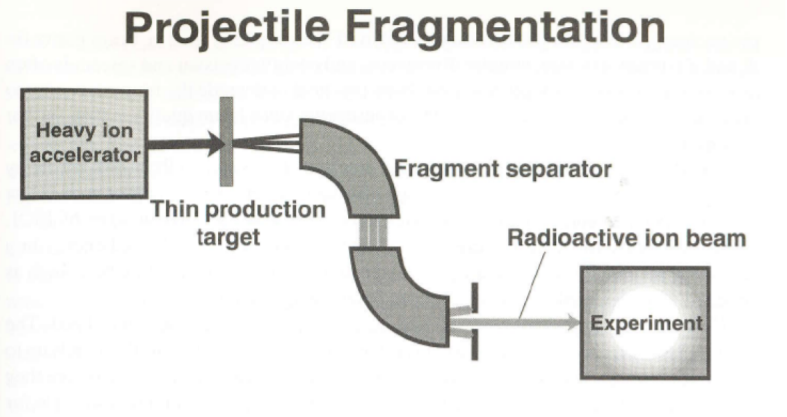
\includegraphics[width=11cm]{NuclearPhysics/modules/nuc-astro/pics/projectile-fragmentation.png}
            \caption{Caption}
            \end{figure}
            
            \textbf{Advantages :} Exotic nuclei are produced wihtout delay (within microseconds) and there is no chemical selectivity\\
            \textbf{Disadvantages :} High energy beam is good for nuclear reactions studies, but too high for many nuclear structure studies.\\
            Shitty beam quaility due to production method.
            
            
        \subsection{Isotope On-Line}
            \indent Light beam (1 GeV p+ or 200 MeV neutrons) on heavy, thick target\\
            Exotic nuclei are produced, thermalize, and are extracted\\
            mass separated\\
            post-accelerated to get radioactive beam\\
            
            
                        
            \begin{figure}[H]
                \centering
                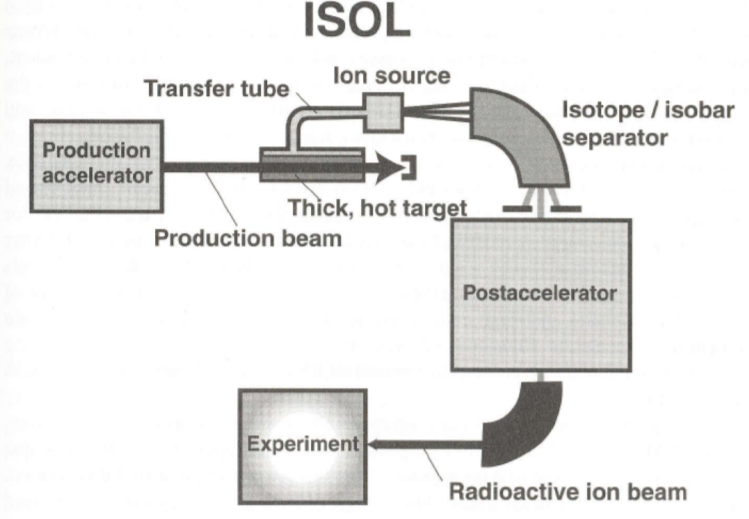
\includegraphics[width=11cm]{NuclearPhysics/modules/nuc-astro/pics/isotope-separator-on-line.png}
            \caption{Caption}
            \end{figure}
         
            \textbf{Advantages :} Lower energy beam (1.5 MeV/A) provides good way to study nuclear structure and astrophysics. \\
            Beam can be selected and then accelerated to desired energy\\
            Very good beam quality (acts like a normal accelerator)\\
            \textbf{Disadvantages :}chemical selectivity within the thick target where isotopes are produced.
         
         
         \subsection{Other Methods}
            Can also get nuclei far from stability by fission of heavy nuclei - spontaneous fission of 252Cf or 235U, or from accelerators - produce proton rich nuclei. 
            
            
    \section{Neutron Stars}
        To be filled out later\\
        Neutron star cooling method:\\
        \href{https://en.wikipedia.org/wiki/Urca_process}{URCA Process}\\
        \href{https://arxiv.org/pdf/astro-ph/0404165.pdf}{Direct URCA Process}\\
        \href{http://news.mit.edu/2018/neutron-stars-protons-may-do-heavy-lifting-0813}{Proton effects in Neutron Stars}\\
        \href{https://en.wikipedia.org/wiki/SN_1987A}{1987 Supernova}\\
        \href{https://en.wikipedia.org/wiki/Neutron_star#Gravity_and_equation_of_state}{Neutron Star EOS}
        
        
        
         
     \begin{figure}[H]
        \centering
        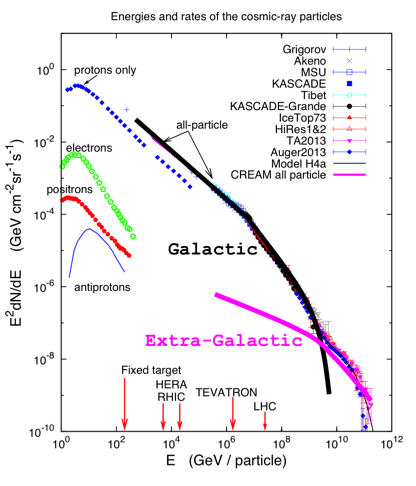
\includegraphics[width=6cm]{NuclearPhysics/modules/nuc-astro/pics/cosmic-ray-flux.png}
        \caption{Caption }
    \end{figure}       
        
        
        
                
         
     \begin{figure}[H]
        \centering
        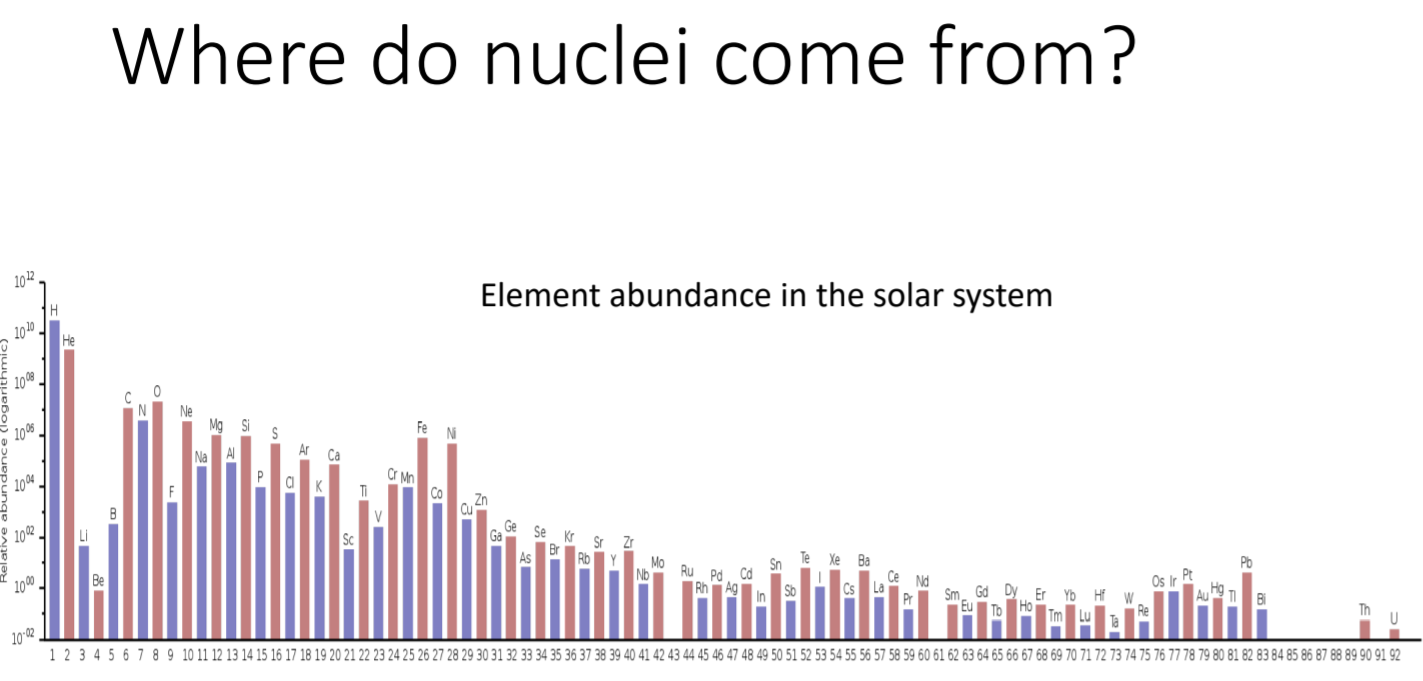
\includegraphics[width=6cm]{NuclearPhysics/modules/nuc-astro/pics/element-abundance.PNG}
        \caption{Caption }
    \end{figure} 



     \begin{figure}[H]
        \centering
        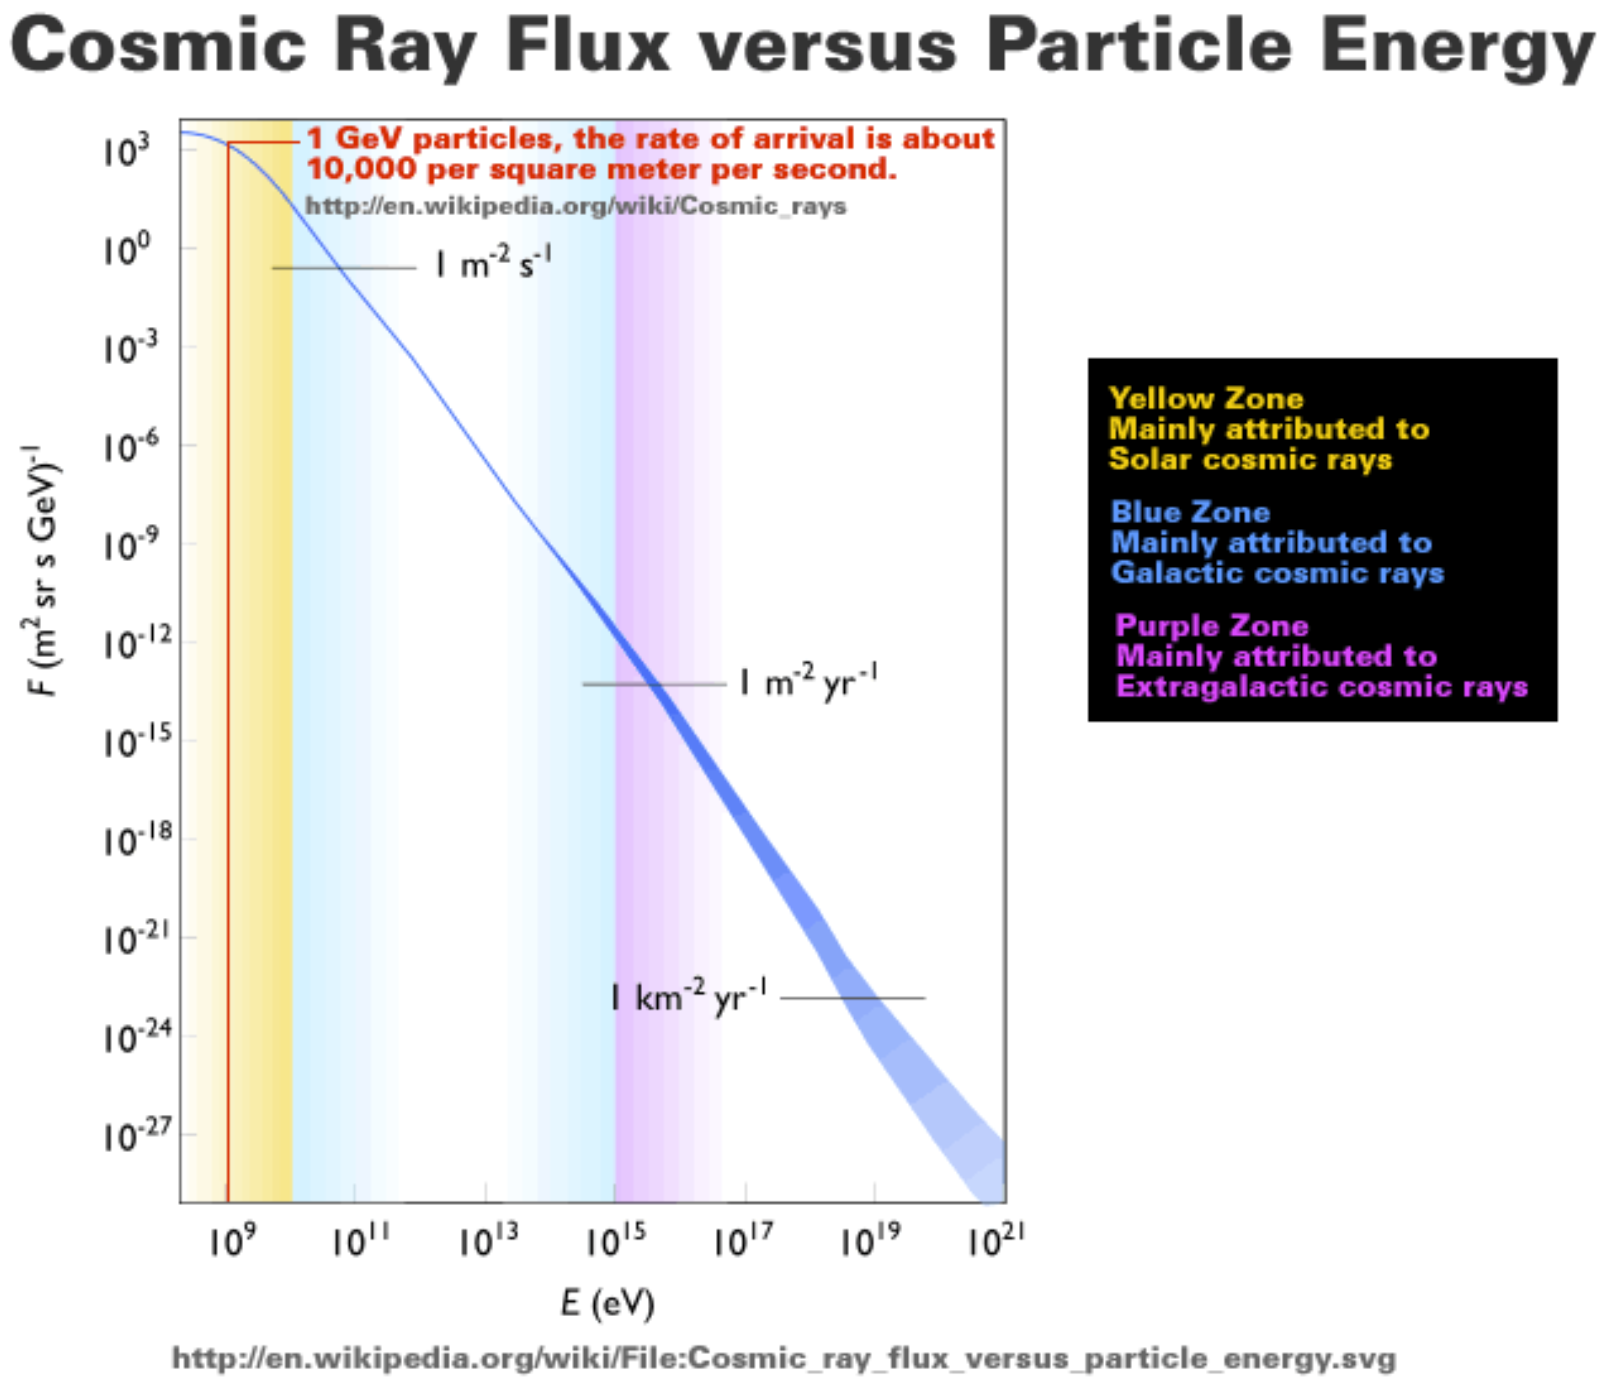
\includegraphics[width=6cm]{NuclearPhysics/modules/nuc-astro/pics/cosmic-ray-flux-log.PNG}
        \caption{Caption }
    \end{figure} 



        
         
     \begin{figure}[H]
        \centering
        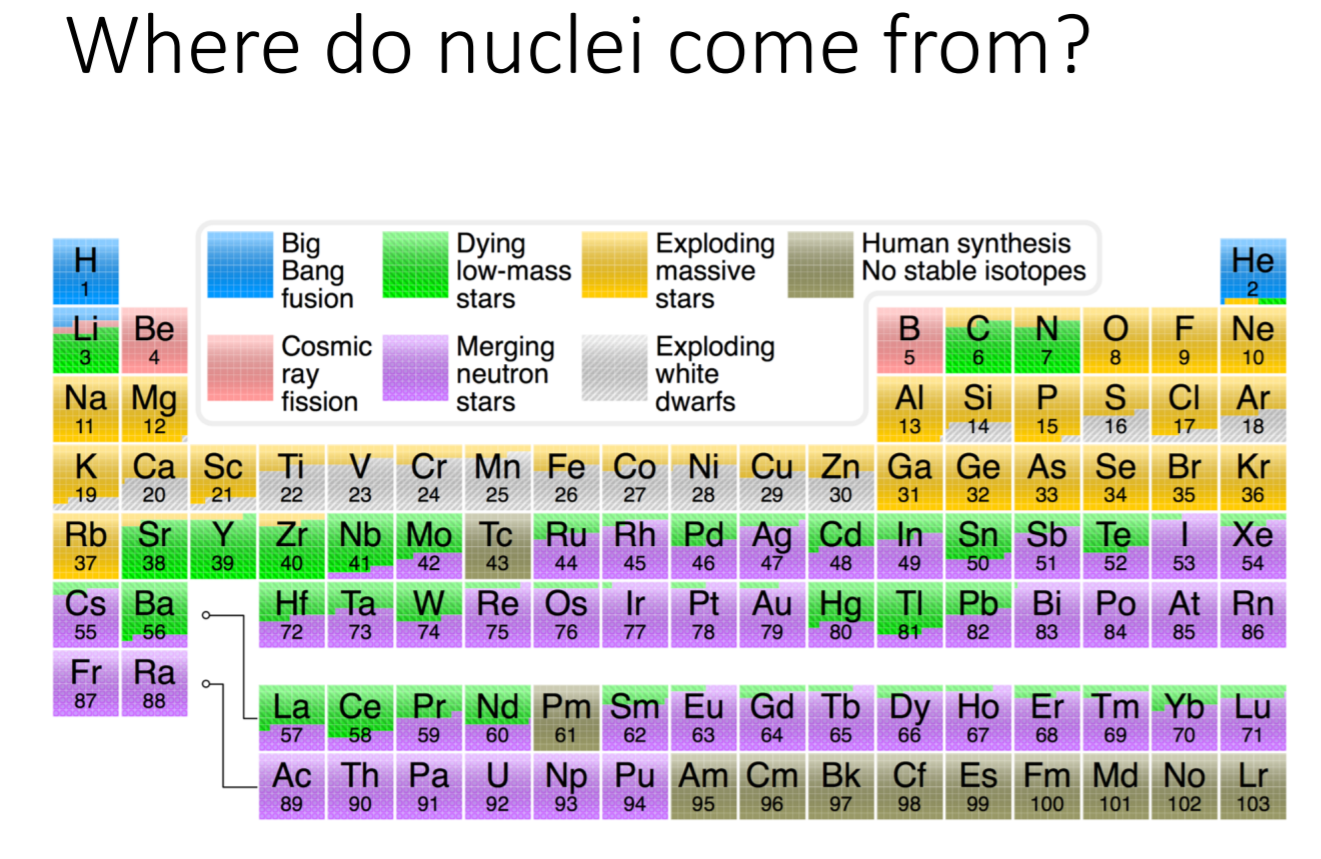
\includegraphics[width=6cm]{NuclearPhysics/modules/nuc-astro/pics/element-origin.PNG}
        \caption{Caption }
    \end{figure} 